% Exemple d'utilisation de la classe `thesul' pour un master.
% D. Roegel, 3/4/2013
%
% Note : les couvertures de Master ne sont pas finalisées dans thesul.
%        Indiquez-moi ce qu'il faut mettre.
%
\documentclass{thesul}

\usepackage{capt-of}
\usepackage{placeins}
\usepackage[toc,page]{appendix}
\usepackage{multirow}
\usepackage{xspace}
\usepackage{latexsym}
\usepackage{amssymb}
\usepackage{listings}
\usepackage{tikz}

\usepackage{color}
\usepackage[T1]{fontenc}

\definecolor{dkgreen}{rgb}{0,0.6,0}
\definecolor{gray}{rgb}{0.5,0.5,0.5}
\definecolor{mauve}{rgb}{0.58,0,0.82}
\definecolor{orange}{rgb}{1.0,0.49,0.0}

\usepackage{enumitem}
\usepackage{pifont}

\lstset{frame=single,
  language={Java},
  aboveskip=3mm,
  belowskip=3mm,
  showstringspaces=false,
  basicstyle={\small\ttfamily},
  numbers=left,
  stepnumber=1,
  numberstyle=\tiny\color{gray},
  keywordstyle=\color{orange},
  commentstyle=\color{dkgreen},
  breaklines=true,
  breakatwhitespace=true,
  tabsize=1,
  morecomment=[l]{\\*},
  morekeywords={}
}
\newcommand\tab[1][1cm]{\hspace*{#1}}
\renewcommand{\floatpagefraction}{.99}
\renewcommand{\textfraction}{.01}

\newcommand{\tlaplus}{TLA\textsuperscript{+}\xspace}
\newcommand{\EXCEPT}{\textsc{except}}
\newcommand{\IF}{\textsc{if}}
\newcommand{\THEN}{\textsc{then}}
\newcommand{\ELSE}{\textsc{else}}
\newcommand{\seq}[1]{\langle #1 \rangle}

\newcommand{\keyword}[1]{\textbf{#1}}
\newcommand{\entity}[1]{\ensuremath{\langle}#1\ensuremath{\rangle}}

% editorial comments in the text or in marginal notes
% 1st argument: initials of the person making the comment,
% 2nd argument: comment to insert
\long\def\ednote#1#2{\par\noindent\framebox{\begin{minipage}{0.99\linewidth}\linespread{.7}\footnotesize #1: #2\end{minipage}}\par}
\newcommand{\edmargin}[2]{\marginpar{\raggedright\linespread{.7}\footnotesize #1: #2}}

%% make TeX use text italic font in math environments
\makeatletter
\newcounter{abr@ctr}
\newcommand{\abr@c}{\c@abr@ctr\advance\c@abr@ctr\@ne}

\DeclareSymbolFont{tlaitalics}{\encodingdefault}{cmr}{m}{it}
\let\itfam\symtlaitalics

\newcommand{\noTeXmath}{%
\c@abr@ctr=\itfam
\multiply\c@abr@ctr"100\relax
\advance\c@abr@ctr "7061\relax
\mathcode`a=\abr@c\mathcode`b=\abr@c\mathcode`c=\abr@c\mathcode`d=\abr@c
\mathcode`e=\abr@c\mathcode`f=\abr@c\mathcode`g=\abr@c\mathcode`h=\abr@c
\mathcode`i=\abr@c\mathcode`j=\abr@c\mathcode`k=\abr@c\mathcode`l=\abr@c
\mathcode`m=\abr@c\mathcode`n=\abr@c\mathcode`o=\abr@c\mathcode`p=\abr@c
\mathcode`q=\abr@c\mathcode`r=\abr@c\mathcode`s=\abr@c\mathcode`t=\abr@c
\mathcode`u=\abr@c\mathcode`v=\abr@c\mathcode`w=\abr@c\mathcode`x=\abr@c
\mathcode`y=\abr@c\mathcode`z=\abr@c
\c@abr@ctr=\itfam
\multiply\c@abr@ctr"100\relax
\advance\c@abr@ctr "7041\relax
\mathcode`A=\abr@c\mathcode`B=\abr@c\mathcode`C=\abr@c\mathcode`D=\abr@c
\mathcode`E=\abr@c\mathcode`F=\abr@c\mathcode`G=\abr@c\mathcode`H=\abr@c
\mathcode`I=\abr@c\mathcode`J=\abr@c\mathcode`K=\abr@c\mathcode`L=\abr@c
\mathcode`M=\abr@c\mathcode`N=\abr@c\mathcode`O=\abr@c\mathcode`P=\abr@c
\mathcode`Q=\abr@c\mathcode`R=\abr@c\mathcode`S=\abr@c\mathcode`T=\abr@c
\mathcode`U=\abr@c\mathcode`V=\abr@c\mathcode`W=\abr@c\mathcode`X=\abr@c
\mathcode`Y=\abr@c\mathcode`Z=\abr@c}

\newcommand{\TeXmath}{%
\mathcode`a="7161\mathcode`b="7162\mathcode`c="7163\mathcode`d="7164%
\mathcode`e="7165\mathcode`f="7166\mathcode`g="7167\mathcode`h="7168%
\mathcode`i="7169\mathcode`j="716A\mathcode`k="716B\mathcode`l="716C%
\mathcode`m="716D\mathcode`n="716E\mathcode`o="716F\mathcode`p="7170%
\mathcode`q="7171\mathcode`r="7172\mathcode`s="7173\mathcode`t="7174%
\mathcode`u="7175\mathcode`v="7176\mathcode`w="7177\mathcode`x="7178%
\mathcode`y="7179\mathcode`z="717A\mathcode`A="7141\mathcode`B="7142%
\mathcode`C="7143\mathcode`D="7144\mathcode`E="7145\mathcode`F="7146%
\mathcode`G="7147\mathcode`H="7148\mathcode`I="7149\mathcode`J="714A%
\mathcode`K="714B\mathcode`L="714C\mathcode`M="714D\mathcode`N="714E%
\mathcode`O="714F\mathcode`P="7150\mathcode`Q="7151\mathcode`R="7152%
\mathcode`S="7153\mathcode`T="7154\mathcode`U="7155\mathcode`V="7156%
\mathcode`W="7157\mathcode`X="7158\mathcode`Y="7159\mathcode`Z="715A}

\tikzstyle{startstop} = [rectangle, rounded corners, minimum width=3cm, minimum height=1cm,text centered, draw=black, fill=red!30]

\tikzstyle{io} = [trapezium, trapezium left angle=70, trapezium right angle=110, minimum width=3cm, minimum height=1cm, text centered, draw=black, fill=blue!30]

\tikzstyle{process} = [rectangle, minimum width=3cm, minimum height=1cm, text centered, draw=black, fill=orange!30]

\tikzstyle{decision} = [diamond, minimum width=3cm, minimum height=1cm, text centered, draw=black, fill=green!30]

\tikzstyle{arrow} = [thick,->,>=stealth]

\noTeXmath
\makeatother

\makeatletter
\newcommand*{\centerfloat}{%
  \parindent \z@
  \leftskip \z@ \@plus 1fil \@minus \textwidth
  \rightskip\leftskip
  \parfillskip \z@skip}
\makeatother

% -------------------------------------------------------------------
%                         Les références
%-------------------------------------------------------------------

\NoChapterNumberInRef
\NoChapterPrefix


\begin{document}

      \OddHead={{\leftmark\rightmark}{\hfil\slshape\rightmark}}
      \EvenHead={{\leftmark}{{\slshape\leftmark}\hfil}}
      \OddFoot={\hfil\thepage}
      \EvenFoot={\thepage\hfil}
      \pagestyle{ThesisHeadingsII}

%-------------------------------------------------------------------
%            Réinitialisation de la numérotation des chapitres
%-------------------------------------------------------------------

% Si la commande suivante est présente,
% elle doit figurer APRÈS \begin{document}
% et avant la première commande \part
\ResetChaptersAtParts 




\MasterUL

\ThesisTitle{Formal Verification of Distributed Algorithms using Distributed PlusCal}
\ThesisAuthor{Heba Al-kayed}

\ThesisPresentedThe{soutenu le 26 juin 2020}
\Encadrants{Stephan Merz, Horatiu Cirstea \\ \tab(VERIDIS)}
\ThesisDomain{Computer Science - MFLS}
\MakeThesisTitlePage
\ThesisFirstPageFoot

%-------------------------------------------------------------------
%                          remerciements
%-------------------------------------------------------------------

%\DontFrameThisInToc
%\begin{ThesisAcknowledgments}
%Les remerciements.
%\end{ThesisAcknowledgments}

%-------------------------------------------------------------------
%                            dédicace
%-------------------------------------------------------------------


%-------------------------------------------------------------------
%                  écriture de `Chapitre' et `Partie' 
%                      dans la table des matières
%-------------------------------------------------------------------

\WritePartLabelInToc
\WriteChapterLabelInToc

%-------------------------------------------------------------------
%                        table des matières
%-------------------------------------------------------------------

\tableofcontents

% Pour ne pas avoir le mot « Chapitre » au début de chaque chapitre.
\NoChapterHead


% La commande \mainmatter permet de passer
% à la numérotation arabe (ce que fait \pagenumbering{arabic}) 
% et de faire commencer la nouvelle page 1 sur une page impaire.
% On évitera donc d'utiliser directement \pagenumbering{arabic}.
\mainmatter


\chapter{Introduction}
%%============================

Distributed systems are based on continuous interactions among components, these interactions produce bugs that are difficult to find by testing as they tend to be non-reproducible or not covered by test-cases.

Distributed systems benefit greatly from testing failure conditions like deadlocks or race conditions at early stages of development at design level.

Formal verification methods have been employed successfully to model the system and its properties and then verify its correctness. One of the verification methods is called model checking \cite{ModelCheckingTLA}, it is a model-based verification technique. Model checking starts with a model described by the user and checks if the properties asserted by the user are valid on that model. 

\tlaplus is a formal languages used to describe algorithms, it provides a flexibility and an expressiveness that enables it to specify and verify complicated algorithms concisely. One of the popular modern examples of incorporating TLA+ to verify distributed algorithms is its usage at Amazon Web Services \cite{amazon}.

Once the user has modeled the system using the \tlaplus specification language, the user can then use the Temporal Logic Checker(TLC) to check both the safety and liveness properties. TLC can further speed-up model checking by running on virtual machines using cloud-based distributed TLC \cite{cloudTLC}. The TLC model checker is offered with the \tlaplus Toolbox. 

In addition, the \tlaplus Toolbox also provides a translator from the algorithmic language PlusCal to \tlaplus. The PlusCal language was designed to provides simple pseudo-code like interface for the user to express concurrent systems. It maintains the expressiveness of \tlaplus while providing the user with a more familiar syntax.

Although PlusCal is very useful, when i comes to distributed algorithms it may enforce some limitation that make it difficult to express them in a natural way. As an example, distributed algorithms usually need to model several sub-processes coexisting and communicating as a part of a distributed node, PlusCal processes must all be declared at top level and cannot be easily used to create what the algorithm is aiming for. 

This thesis proposes Distributed PlusCal, an extension of PlusCal that introduces constructs that can overcome these limitation. Distributed PlusCal is a language that provides algorithm designers with an interface in which distributed algorithms and their properties can be expressed naturally.

Our motivations for creating Disrtibuted PlusCal are quite similar to the motivations that created PlusCal, we want a syntax that would spare the user from having to model primitives that usually accompany distributed algorithms.


\chapter{Background info}
%%============================

This chapter is an overview of TLA+ and PlusCal.
\section{\tlaplus}
%%============================

\tlaplus is a formal specification language in which algorithms and systems can be described at a high level of abstraction and can be formally verified using the model checker TLC or the interactive proof assistant TLAPS. \tlaplus is based on mathematical set theory for describing data structures in terms of sets and functions, and on the Temporal Logic of Actions TLA for specifying their executions as state machines. \tlaplus specifications usually have the form
\[
  Init \land \Box[Next]_{vars} \land L
\]
where $Init$ is a predicate describing the possible initial states, $Next$ is a predicate that constrains the possible state transitions, $vars$ is the tuple of all state variables that appear in the specification, and $L$ is a liveness or fairness property expressed as a formula of temporal logic. Transition formulas such as $Next$, also called \emph{actions}, are at the core of \tlaplus, and represent instantaneous state changes. They contain unprimed state variables denoting the value of the variable before the transition as well as primed state variables that denote the value after the transition.

\begin{figure}
\begin{lstlisting}% [caption = A memory specification in \tlaplus., frame = tlrb, firstnumber =  1,label=memory-tla]

---------------------------- MODULE SimpleMemory ----------------------------
CONSTANTS Address, Value, InitValue, NoValue

ASSUME 
  /\ InitValue \in Value
  /\ NoValue \notin Value

VARIABLES chan, mem

\* initial condition
Init == 
  /\ chan = NoValue
  /\ mem = [a \in Address |-> InitValue]

\* transitions: reading and writing
Read(a) == 
  /\ chan' = mem[a]
  /\ mem' = mem

Write(a,v) ==
  /\ mem' = [mem EXCEPT ![a] = v]
  /\ chan' = NoValue

Next ==
  \/ \E a \in Address : Read(a)
  \/ \E a \in Address, v \in Value : Write(a,v)

\* overall specification
Spec == Init /\ [][Next]_<<chan,mem>>

\* predicate specifying type correctness
TypeOK == 
  /\ chan \in Value \cup {NoValue}
  /\ mem \in [Address -> Value] 
=============================================================================
\end{lstlisting}
\caption{A memory specification in \tlaplus.}
\label{memory-tla}
\end{figure}

For example, figure~\ref{memory-tla} shows a \tlaplus specification of a simple memory. It declares four constant parameters $Address$, $Value$, $InitValue$, and $NoValue$, and states a hypothesis on the values that these parameters can be instantiated with. The state space of the specification is represented by the two variables $chan$ and $mem$. Intuitively, $mem$ holds the current memory, whereas $chan$ is an output channel that reflects the result of the preceding operation.

The remainder of the \tlaplus module contains operator definitions that represent parts of the specification and of correctness properties. The state predicate $Init$ fixes the initial values of the two variables. The actions $Read(a)$ and $Write(a,v)$ represent reading the value at memory address $a$ and writing value $v$ to memory address $a$, respectively. In this specification, the memory is modeled as a function mapping addresses to values. The \tlaplus expression $[x \in S \mapsto e]$ denotes the function with domain $S$ such that every element $x$ of $S$ is mapped to $e$. This is reminiscent of a $\lambda$-expression but also makes explicit the domain of the function. Function application $f[x]$ is written using square brackets. Finally, the expression $[f\ \EXCEPT\ ![x] = e]$ denotes the function that is similar to $f$, except that argument $x$ is mapped to $e$, one can think of it as a function overwrite.

The action $Next$ defines the possible state transitions as the disjunction of $Read$ and $Write$ actions, and $Spec$ represents the overall specification of the memory.

\tlaplus is an untyped language. Type correctness can be verified as a property of the specification. For our example, the predicate $TypeOK$ indicates the possible values that the variables $chan$ and $mem$ are expected to hold at any state of the specification. Formally, the implication $Spec \Rightarrow \Box TypeOK$ can be established as a theorem.

\bigskip


For More details on the syntax and grammer of TLA+, see \cite{tlabook} \cite{tlaplus}.

\section{PlusCal algorithm language}
%%============================

\tlaplus is a specification formalism not a programming language. It relies on mathematical logic and formulas for structuring specifications, which may discourage programmers from using it. PlusCal~\cite{pcalAlgo} was designed as an algorithm language with a more familiar syntax that can be translated into \tlaplus specifications and then be verified using the familiar \tlaplus tools.

An algorithm language is used to focus on aspects of the algorithm such as data manipulation rather than irrelevant and distracting details that involve programming-language objects and data structures.
	
PlusCal is an algorithm language that describes both concurrent and sequential algorithms, it maintains the expressiveness of \tlaplus as well as representing atomicity conveniently.

The TLA+ Toolbox provides a platform where algorithm designers can model their algorithms using PlusCal, translate them to the corresponding \tlaplus specifications and check for the algorithm's correctness through the TLC model checker.

A PlusCal algorithm is located in a comment statement within the \tlaplus module. The general structure of a PlusCal algorithm is shown in Figure \ref{pluscal-struct}.

\begin{figure}[!h]
\begin{lstlisting}% [caption = General structure of a PlusCal algorithm, frame = tlrb, firstnumber =  1,label=pluscal-struct]

(** algorithm <algorithm name>

(* Declaration section *)
variables <variable declarations>

(* Definition section *)
define <definition name> == <definition description>

(* Macro section *)
macro <name>(var1, ...)
 <macro body of statements>

(* Procedure section *)
procedure <name>(arg1, ...)
 variables <local variable declarations>
 <procedure body of statements>

(* Processes section *)
process (<name> [=|\in] <expr>))
  variables <variable declarations>
  <process body of statements>

**)

\end{lstlisting}
\caption{General structure of a PlusCal algorithm}
\label{pluscal-struct}
\end{figure}

The \textbf{Declaration section} is where the user declares global variables that are shared among all the components of the algorithm. The \textbf{Definition section} allows the user to write TLA+ definitions of operators that may refer to the algorithm's global variables.
The \textbf{Macro section} holds macros whose bodies are expanded at translation time incorporating the parameters passed from the calling statement, similar to the expansion of C pre-processing macros. A \textbf{procedure} in PlusCal take a number of arguments, can declare local variables, and can modify the global variables; it does not return a result. A \textbf{process} begins in one of two ways: 
\begin{center}
$process (ProcName \in IdSet)$ \\
$process (ProcName = Id)$
\end{center}

The first form declares a set of processes, the second an individual process. these statements are optionally followed by declarations of local variables. The process body is a sequence of statements, within the body of a process set, $self$ equals the current process's identifier.

Procedure and process bodies may contain labels. All PlusCal statements appearing between two labels are executed atomically, and certain rules determine where labels must and may not appear.
PlusCal enforces a strict ordering of its blocks. The define block has to come before any macros, which has to come before any procedures, which has to come before any processes. The full grammar of the PlusCal algorithm language can be found in appendix A of the PlusCal manual~\cite{pcalAlgo}.

Figure \ref{semaphoreEx} shows the modeling of a semaphore mutex example in PlusCal, Semaphores are integer variables that are used to solve the critical section problem.

\FloatBarrier 
\begin{figure}
\begin{lstlisting}[frame = tlrb, firstnumber = 1]
(*
--algorithm SemaphoreMutex {
variables sem = 1;
 
  process(p \in 1..N)
  {
  start : while (TRUE){
  enter :    when (sem > 0);
                  sem := sem - 1;            
  cs :       skip ;
  exit :     sem := sem + 1 ;
          }
  }
}
*)

\end{lstlisting}
\caption{Semaphore mutex example in PlusCal}
\label{semaphoreEx}
\end{figure} 

\paragraph{Translation to \tlaplus.}
The PlusCal translator expects as input a PlusCal algorithm following the structure described previously.

The translator parses the PlusCal algorithm and generates the corresponding \tlaplus specification in roughly the following steps.

\begin{enumerate}
\item Generate all the definitions and variables regardless of their scope within the PlusCal algorithm, as well as $vars$ the tuple of all variables.
The $pc$ variable is introduced by the translator to track the control flow of processes.

\FloatBarrier
\begin{lstlisting}[frame = tlrb, firstnumber = 1,xleftmargin=.2\textwidth, xrightmargin=.2\textwidth]
\* BEGIN TRANSLATION
VARIABLES sem, pc

vars == << sem, pc >>

\end{lstlisting}

\item Generate $ProcSet$ which is a set that contains all the process identifiers.

\begin{lstlisting}[frame = tlrb, firstnumber = 1,xleftmargin=.2\textwidth, xrightmargin=.2\textwidth]
ProcSet == (1..N)

\end{lstlisting}

\item  Generate $Init$, the initial predicate that specifies the initial values of all the declared variables. Comments indicate if the variables are global or local to a process or procedure.
The variable $pc$ is defined and used as a program control variable, it's a function whose domain is $ProcSet$ such that each element is mapped to the entry label of the process.

\begin{lstlisting}[frame = tlrb, firstnumber = 1, xleftmargin=.2\textwidth, xrightmargin=.2\textwidth]
Init == (* Global variables *)
        /\ sem = 1
        /\ pc = [self \in ProcSet |-> "start"]

\end{lstlisting}

\item For each PlusCal label, generate a \tlaplus action that represents the atomic operation beginning at that label. 
In the produced actions unprimed variables refer to their values before executing the action and the primed variables refer to their values after the execution.
The definition is parameterized by the identifier $self$,
which represents the identifier for the current process. For example, the following action is generated for label \texttt{enter} of the semaphore algorithm.

\begin{lstlisting}[frame = tlrb, firstnumber = 1, xleftmargin=.2\textwidth, xrightmargin=.2\textwidth]
enter(self) == /\ pc[self] = "enter"
               /\ (sem > 0)
               /\ sem' = sem - 1
               /\ pc' = [pc EXCEPT ![self] = "cs"]
\end{lstlisting}

Moreover, the PlusCal translator generates an action that corresponds to the disjunction of the actions for the individual labels and that represents the transition relation of a process.

\begin{lstlisting}[frame = tlrb, firstnumber = 1, xleftmargin=.05\textwidth, xrightmargin=.05\textwidth]
p(self) == start(self) \/ enter(self) \/ cs(self) \/ exit(self)
\end{lstlisting}

\item Generate the next-state action $Next$ that constrains the possible state transitions, and the complete specification $Spec$.

\begin{lstlisting}[frame = tlrb, firstnumber = 1, xleftmargin=.2\textwidth, xrightmargin=.2\textwidth]
Next == (\E self \in 1..N: p(self))

Spec == Init /\ [][Next]_vars

\end{lstlisting}

\end{enumerate}


In practice, to use PlusCal the user must understand the generated TLA+ specifications, in order to write the properties in terms of the TLA+ variables introduced by the compiler.

A more detailed description of the translation strategy can be found in \cite{pcalAlgo}.

\chapter{Related work}
%%============================

There are several modeling languages that are used to specify algorithms and then verify them with the help of a model checker. Modular PlusCal \cite{ModularPlusCal} is an extension of PlusCal that aims to add the ability to specify an interface between the actual substance of a PlusCal algorithm and the environment.

Modular PlusCal is a part of a tool called PGo \cite{PGO}, PGO produces an implementation in Go(C based language developed by Google) based on a PlusCal/TLA+ specification.

\section{PGO}

PGo is a source to source compiler written in Java. PGo can compile Modular PlusCal to PlusCal, PlusCal to Go, and Modular PlusCal to Go.

\subsection{Modular PlusCal}

Modular PlusCal is an extension of PlusCal, using Modular PlusCal the user can separate the specification into two components, a system functionality specification concerned with what the algorithm is supposed to achieve, and an environment specification concerned about how we may want it achieved. Modular PlusCal allows the user to separate abstract and implementation-dependent details.
\hfill\\

For example, if we consider a server/client based communication system, where the system functionality is a client requesting services, then the fact that the client is requesting the service via a TCP connection is called an environment specification. 
An added value for this separation is that the programmer can reuse concepts defined in one specification in another specification, since the environment specification isn't dependent on the functionality of the system.

Modular PlusCal is compiled by PGo to PlusCal, which is then translated to \tlaplus by the help of the \tlaplus toolbox. Modular PlusCal introduced archetypes, mapping macros, and instances to achieve the modularization of the spec.

\paragraph{\textbf{Architypes}}
\hfill\\
Architypes are considered to be the blue print of a PlusCal process, they are used to specify the system behaviors. They have the same semantics except for the inability to access global variables unless passed to the architypes as arguments.

An archetype must communicate with its environment via a set
of parameters that it accepts. Instead of specifying shared global variables.

They are capable of both input and output due to the 'pass by reference' parameters, using the \textit{ref} keyword before a global variable that is sent as an argument lets us know that this architype can modify it.

The syntax is similar to the syntax for a PlusCal process; however, an architype is not allowed to access to global variables that are out of its scope. An archetype should never rely on anything that is not explicitly passed to it as a parameter. These restrictions provide the needed isolation between system and environment behaviors.

\paragraph{Mapping Macros}

Mapping Macros specify the environment, they define interfaces for reading and writing on a global variable that represents a network. Like PlusCal all statements in a macro are part of the same atomic step, therefore labels are not allowed within a mapping macro.

Modeling mapping macros independently from system functionality allows the user to reuse the mapping macros.

\paragraph{Instances}

Instances are the glue that holds the archtypes and mapping macros together.Instances instantiate a process or a group of processes using the specified architype, where each argument passed to the architype is bound with a mapping macro to control read and write functions on it.


\chapter{Distributed PlusCal}

Distributed PlusCal is a language used to describe distributed algorithms, it extends PlusCal. 
Our motivations for creating Disrtibuted PlusCal are quite similar to the motivations that created PlusCal, we want a syntax that would spare the user from having to model primitives that usually accompany distributed algorithms.

Since we extended the existing PlusCal translator responsible for parsing PlusCal into TLA+ we inherited the same semantics and grammar and added our own.

\section{Structure of an algorithm}

The general structure and organization of a Distributed PlusCal algorithm is shown in Figure \ref{dpluscal-struct}.


\begin{figure}
\begin{lstlisting}% [caption = General structure of a Distributed PlusCal algorithm, frame = tlrb, firstnumber =  1,label=dpluscal-struct]

(* PlusCal options section *)
(* PlusCal options (-distpcal) *)

(* algorithm <algorithm name>

(* Declaration section *)
variables <variable declarations>
channels <channel declarations>
fifos <fifo declarations>

(* Definition section *)
define <definition name> == <definition description>

(* Macro section *)
macro <name>(var1, ...)
 <macro-body of statements>

(* Procedure section *)
procedure <name>(arg1, ...)
 variables <local variable declarations>
 <procedure body of statements>

(* Processes section *)
process (<name> [=|\in] <Expr>))
  variables <variable declarations>
  <sub-processes>

*)

\end{lstlisting}
\caption{General structure of a Distributed PlusCal algorithm}
\label{dpluscal-struct}
\end{figure}

\textbf{PlusCal options section} holds options to be passed to the translator, for example adding $-label$ to the PlusCal options turns on the automatic labeling of the algorithm by the translator. Since we extended the PlusCal translator we notify the translator to parse a Distributed PlusCal algorithm by passing the $-distpcal$ option.\\

Figure \ref{dpluscal-struct} resembles figure \ref{pluscal-struct}, however the variable declarations in the \textbf{declarations section} enables the user to declare primitive constructs such as non-ordered channels and FIFO based channels in addition to PlusCal variables.More details on the communication channels are available in section \ref{comChannels}.

In the \textbf{Process Section} the process can hold multiple sub-processes each with it's own body of statements.More details on the sub-processes are available in section \ref{subProcess}.


\hfill\\
In the sections that follow we will be doing a walk-through on the two phase commit protocol \ref{appendix:examples}, it is used in distributed transactions that consist of multiple operations, performed at multiple sites. The goal of the protocol is to reach consensus between the different elements that carry out the transaction together such that if an element decides to abort all other elements abort as well, and the transaction is rolled back.

\FloatBarrier
\section{Communication Channels}
\label{comChannels}

Distributed algorithms composed of multiple processes communicate by exchanging messages through channels. Channels provide communication and coordination for distributed applications. They are classified by the way they handle the addition and removal of messages from their collections. 

For some algorithms message ordering is critical, for example if a message is sent to subscribe in a service and another is send to unsubscribe, it is crucial that the first message is received and handled before the second. However, some algorithms are not dependent on ordering. Distributed PlusCal offers two types of channels, unordered channels as well as FIFO based channels.

Channels in Distributed PlusCal are unbounded , meaning there is no maximum capacity for the messages they can hold.

The sections to follow explain how to define and use the channels as well as their \tlaplus translations. 

\subsection{Unordered Channels}

Unordered channels are declared and used as communication gateways in algorithms that are not dependent on the order in which the messages are handled.

The general structure for channel declaration is shown below. An unordered channel is declared with the keyword \keyword{channel} or \keyword{channels}. 

\[
 \keyword{channel}\ \entity{identifier}[\entity{dimention1,...,dimentionN}];
\]

The equivalent PlusCal declaration of the same channel would be as follows

\[
 \keyword{variable}\ \entity{identifier}[\entity{d1 \in dimention1,... dN \in dimentionN |-> \{\}}];
\]

The $dimensions$ are \tlaplus sets that are defined in the \tlaplus file, they represent the keys of the channel, Figure \ref{unorderedtla} shows the corresponding TLA+ translation of the unordered channel declaration with N dimensions.


The TLA+ translation of the FIFO channel is as follows

\[
 \entity{identifier} = [\entity{d1 \in dimention1,... dN \in dimentionN |-> \{ \}}];
\]

In our two phase commit example, we have two unordered channels $coord$ and $agt$.The channel $agt$ has a dimension composed of the values of the set $Agent$, the set $Agent$ is a constant in our algorithm. The Distributed PlusCal declarations and \tlaplus translation are in Figure \ref{2pcchannels}.


\FloatBarrier
\begin{figure}[!h]

\begin{minipage}{.3\textwidth}

\lstinline|channels coord, agt[Agent]| $\triangleq$ \\\\
\end{minipage}\hfill
\begin{minipage}{.7\textwidth}
\begin{lstlisting}[frame = none, numbers = none]
Init == (* Global variables *)
        /\ coord = {}
        /\ agt = [a0 \in Agent |-> {}]
\end{lstlisting}

\end{minipage}\hfill

\caption{Unordered channel declaration - TLA+ translation example}
\label{2pcchannels}
\end{figure}
\FloatBarrier

Unordered channel are represented by \tlaplus sets. \tlaplus sets are the basic construct for representing data. Sets are not concerned with the order of elements within their collection.

Set operators include $\in$ which is written as \lstinline|\in| in \tlaplus checks whether an element is a part of a set, $\cup$ is written as \lstinline|\cup| adds an element to the set.

Distributed PlusCal extended PlusCals allowed statements within a body to include channel operators.

The list below shows the syntax of the channel operators and their \tlaplus translations, to simplify the examples assume we are dealing with a one-dimensional channel (indexed by set $IdSet$) with the identifier $chan$.

\begin{itemize}
\item[$\Diamond$]  \textbf{send} The $send$ operator carries two parameters, the channel $chan$ and the message $msg$. The purpose of this operator is to add the message $msg$ to
the given channel. Since the unordered channel is represented using a \tlaplus set, addition to a set is performed using the set operator $\cup$ which is written in \tlaplus as \lstinline|\cup|.


\begin{minipage}{.24\textwidth}

\lstinline|send(chan[e], msg)| $\triangleq$
\end{minipage}\hfill
\begin{minipage}{\textwidth}
\begin{lstlisting}[frame = none, numbers = none]
chan' = [chan EXCEPT ![e] = chan[e] \cup {msg}]
\end{lstlisting}

\end{minipage}\hfill

\item[$\Diamond$]  \textbf{broadcast}

The $broadcast$ operator takes two parameters, the channel $chan$ and the message $msg$. The purpose of this operator is to add the message $msg$ to every element of the given channel.

\begin{minipage}{.25\textwidth}

\lstinline|broadcast(chan, msg)| $\triangleq$
\end{minipage}\hfill
\begin{minipage}{.8\textwidth}
\begin{lstlisting}[frame = none, numbers = none]
chan' = [el \in IdSet |->chan[el] \cup {msg}]
\end{lstlisting}

\end{minipage}\hfill

Note that we don't specify an element when referring to the channel in the first argunemt, as the message is meant to be sent to all elements.
\item[$\Diamond$] \textbf{multicast}

The $multicast$ operator takes two parameters, the channel $chan$ and a \tlaplus expression. The second parameter specifies the intended recipients in the channel and the message. The purpose of this operator is to identify the recipients such that if they fall within the required subset, the message is added to their sets; otherwise, their sets remain unchanged.

\begin{minipage}{.4\textwidth}

\lstinline!multicast(chan, [a \in sub |-> msg])! $\triangleq$\\\\\\
\end{minipage}\hfill
\begin{minipage}{.8\textwidth}
\begin{lstlisting}[frame = none, numbers = none]
chan' = [a \in DOMAIN chan |-> 
					IF a \in sub
					THEN chan[a] \cup {msg}
					ELSE chan[a]]
\end{lstlisting}

\end{minipage}\hfill

\item[$\Diamond$]  \textbf{receive}
The $receive$ operator has two parameters, the channel $chan$ and a \tlaplus variable $var$. The purpose of this operator is to remove an element from the channel and add it to the variable sent in the second argument.

\begin{minipage}{.33\textwidth}

\lstinline|receive(chan[element], var)| $\triangleq$\\\\
\end{minipage}\hfill
\begin{minipage}{\textwidth}
\begin{lstlisting}[frame = none, numbers = none]
\E e \in chan[element]:
   /\ var' = e
   /\ chan' = [chan EXCEPT ![element] = chan[element] \ {e}]
\end{lstlisting}

\end{minipage}\hfill

\item[$\Diamond$]  \textbf{clear}
The $clear$ operator empties the channel $chan$.

\lstinline|clear(chan)| $\triangleq$
\lstinline|chan' = [el \in IdSet -> {}]|

\end{itemize}

The two phase commit example in \ref{appendix:examples} includes the functions $send$, $broadcast$, $receive$ and $clear$ with their \tlaplus translations. The listings below focus on the $send$ and $receive$ operations.

In the example, an agent process decides whether it wants to "accept" or "refuse" a transaction and the decision is held by the variable $st$, then the process informs the coordinator of its decision through the channel $coord$.

\begin{minipage}{.46\textwidth}

\lstinline!send(coord, [type |-> st, agent |-> self])! $\triangleq$
\end{minipage}
\begin{minipage}{.9\textwidth}
\lstinline!coord' = (coord \cup {[type |-> st, agent |-> self]})!
\end{minipage}\hfill\hfill

The coordinator receives the decisions of the agents though the $coord$ channel, the translation consists of first ensuring that the channel is not empty, then removing an element from the channel and placing it in the variable of the second argument. 

\begin{minipage}{.25\textwidth}

\lstinline!receive(coord, msg)! $\triangleq$\\\\
\end{minipage}
\begin{minipage}{.9\textwidth}
\begin{lstlisting}[frame = none, numbers = none]
\E c \in coord:
	/\ coord' = coord \ {c}
	/\ msg' = c
\end{lstlisting}

\end{minipage}\hfill


\subsection{FIFO channels}

FIFO channels are declared and used for algorithms whose correctness depends on handling the messages in the order of their creation.

The general structure for channel declaration is shown below. A FIFO channel is declared with the keyword \keyword{fifo} or \keyword{fifos}. 

\[
 \keyword{fifo}\ \entity{identifier}[\entity{dimention1,...,dimentionN}];
\]

The equivalent PlusCal declaration of the same channel would be as follows

\[
 \keyword{variable}\ \entity{identifier}[\entity{d1 \in dimention1,... dN \in dimentionN |-> \seq{}}];
\]

The TLA+ translation a FIFO channel is as follows

\[
 \entity{identifier} = [\entity{d1 \in dimention1,... dN \in dimentionN |-> \seq{}}];
\]


FIFO channels are represented as \tlaplus sequences.
\tlaplus sequences are ordered collections, analogous to lists. Adding to a sequence corresponds to appending at the end of the sequence with the $Append$ operator, and removing the first element of a sequence can be accomplished with the $Tail$ operation. We take advantage of these operators to maintain the order in the FIFO channels.

All sequences are \tlaplus functions, where $\seq{}$ represents an empty sequence.

Appendix \ref{appendix:examples} includes an example for  modeling Lamports Mutual Exclusion algorithm, an algorithm that uses time stamps to order critical section requests and to resolve any conflict between requests. The example introduces a two dimensional FIFO channel $network$, the dimensions are sets introduced on the algorithm.

The Distributed PlusCal declaration and the \tlaplus translation of the $network$ FIFO channel are in Figure \ref{fifochannels}.
 

\FloatBarrier
\begin{figure}[!h]
\begin{minipage}{.3\textwidth}

\lstinline|fifo network[Nodes, Nodes]| $\triangleq$ 
\end{minipage}\hfill
\begin{minipage}{.7\textwidth}
\begin{lstlisting}[escapechar=\%, frame = none, numbers = none]
network = [n0 \in Nodes, n1 \in Nodes |-> %$\seq{}$%]
  
\end{lstlisting}  
\end{minipage}\hfill
\caption{FIFO channel declaration - TLA+ translation}
\label{fifochannels}
\end{figure}
\FloatBarrier


Distributed PlusCal added to the statements allowed within a body functions that are applied on channels.
The list below shows the syntax of the channel operators and their \tlaplus translations, to simplify the examples assume we are dealing with a one dimensional channel (indexed by $IdSet$) with the identifier $chan$.

\begin{itemize}

\item[$\Diamond$]  \textbf{send} The $send$ operator carries two parameters, the channel $chan$ and the message $msg$. The purpose of this operator is to add the message $msg$ to
the given channel. Since the FIFO channel is represented using a \tlaplus sequence, addition to a sequence is performed using the operator $Append$ which adds to the tail of the sequence.

\begin{minipage}{.25\textwidth}

\lstinline|send(chan[e], msg)| $\triangleq$
\end{minipage}\hfill
\begin{minipage}{\textwidth}
\begin{lstlisting}[frame = none, numbers = none]
chan' = [chan EXCEPT ![e] = Append(@, msg)]
\end{lstlisting}

\end{minipage}\hfill

\item[$\Diamond$]  \textbf{broadcast}
The $broadcast$ operator takes two parameters, the channel $chan$ and the message $msg$. The purpose of this operator is to add the message $msg$ to every element of the given channel.

\begin{minipage}{.25\textwidth}

\lstinline|broadcast(chan, msg) | $\triangleq$
\end{minipage}\hfill
\begin{minipage}{.7\textwidth}
\begin{lstlisting}[frame = none, numbers = none]
chan' = [el \in IdSet -> Append(chan[el], msg)]
\end{lstlisting}

\end{minipage}\hfill

\item[$\Diamond$] \textbf{multicast}

The $multicast$ operator takes two parameters, the channel $chan$ and a \tlaplus expression. The second parameter specifies the intended recipients in the channel and the message. The purpose of this operator is to identify the recipients such that if they fall within the required subset, the message is added to their sets; otherwise, their sets remain unchanged.

\begin{minipage}{.44\textwidth}

\lstinline!multicast(chan, [a \in sub |-> msg])! $\triangleq$\\\\\\
\end{minipage}\hfill
\begin{minipage}{.6\textwidth}
\begin{lstlisting}[frame = none, numbers = none]
chan'=[a \in DOMAIN chan 
			|-> IF a \in sub 
       THEN Append(chan[a], msg)
       ELSE chan[a]]
\end{lstlisting}

\end{minipage}\hfill


\item[$\Diamond$]  \textbf{receive}

The $receive$ operator has two parameters, the channel $chan$ and a \tlaplus variable $var$. The purpose of this operator is to remove the first element from the channel using the $Head$ and $Tail$ operators and add it to the variable sent in the second argument.

\begin{minipage}{.3\textwidth}

\lstinline|receive(chan[e],var)| $\triangleq$\\\\
\end{minipage}\hfill
\begin{minipage}{.7\textwidth}
\begin{lstlisting}[frame = none, numbers = none]
/\ Len(chan[e]) > 0 
/\ var' = [Head(chan[e])]
/\ chan' = [chan EXCEPT ![e] =  Tail(@) ]
\end{lstlisting}

\end{minipage}\hfill

\item[$\Diamond$]  \textbf{clear}
The $clear$ operator empties the channel $chan$.

\begin{center}

\lstinline|clear(chan)| $\triangleq$
\lstinline|chan' = [el \in IdSet -> $\seq{}$$\seq{}$]|

\end{center}
\end{itemize}

The Lamport Mutex example in \ref{appendix:examples} includes the operators $send$, $multicast$, $receive$ and $clear$ with their \tlaplus translations. The listings below focus on the $receive$ operation as an example.


In the example, $Nodes$ represent a set with all the nodes in our algorithm. The channel $network[Nodes,Nodes]$ represents a channel where the first dimension is a sender node and the second dimension is a receiver node. When a process receives from the channel $network[n,self]$ where $n \in Nodes$, the channel is receiving messages sent for it.

The \tlaplus translation use the operators $Head$ and $Tail$ in order to read the first element in the channel and remove it as well.

\begin{minipage}{.35\textwidth}

\lstinline!receive(network[n,self], msg)! $\triangleq$\\\\
\end{minipage}
\begin{minipage}{\textwidth}
\begin{lstlisting}[frame = none, numbers = none]
/\ Len(network[n,self]) > 0 
/\ msg' = [msg EXCEPT ![self] = Head(network[n,self])]
/\ network' = [network EXCEPT ![n,self] =  Tail(@) ]
\end{lstlisting}
\end{minipage}\hfill\hfill


\section{Sub-Processes}
\label{subProcess}

Distributed PlusCal gives the user the opportunity to define multiple sub-processes per process. Each sub-process consists of labeled statements. Essentially this enables the process to execute multiple tasks in parallel.

The body of a sub-process maintains the same syntax as the body of a PlusCal process. All the sub-processes share the same variables declared for the process, this makes communication between them possible if needed.

The Figure \ref{2pcSub} shows a sub-process defined for the two phase commit algorithm, the example is written in c-syntax and the sub-processes are surrounded by curly braces.
The entire algorithm is in Appendix \ref{appendix:examples}.

\begin{figure}[!h]
\label{2pcSub}
\begin{lstlisting}[caption = Distributed PlusCal Sub-Processes, frame = tlrb, firstnumber = 1]
   
  fair process (a \in Agent)
  variable aState = "unknown"; { \* sub-process

a1: if (aState = "unknown") {
        with(st \in {"accept", "refuse"}) {
          aState := st;
          send(coord, [type |-> st, agent |-> self]);
        };
    };
    a2: await(aState \in {"commit", "abort"})
    
  } { \* sub-process
    
    a3:await (aState # "unknown");
       receive(agt[self], aState); 
       
    a4:clear(agt);
  }

\end{lstlisting}
\end{figure}

\hfill\\

The process represents an Agent process that communicates with a coordinator in order to apply a decision. The process consists of two sub-processes, where the first sub-process contains the atomic labels <<a1, a2>> and the second sub-process contains <<a3, a4>>.

it's important to note that the sub-processes do not allow variable declarations they only use variables declared for the entire process.

\subsection{TLA+ Translation}

The translation of a Distributed PlusCal process into TLA+ meant having to introduce structures and sets that refer to the sub-processes as well as the processes.

Initially a set \textbf{SubProcSet} was added to hold all the sub-process identifiers, with respect to which process they belonged to.

\[
SubProcSet \triangleq [P \in ProcSet \mapsto \IF\ P \in IdSet\ \THEN\  1..n\ 
								\ELSE\  1..m ]
\]						  

The value of the \textbf{pc} variable in PlusCal is a single string equal to the label of the next statement to be executed with respect to a process. In Distributed PlusCal we extended the definition to indicate which sub-process is involved as well.

Since in \tlaplus a function with domain $1..n$ for some $n \in Nat$ is a sequence, the $pc$ variable in Distributed PlusCal is initialized as

\[
pc = [self \in ProcSet \mapsto [self \in IdSet \mapsto \seq{"lbl",\dots}]]
\]	

where the labels that appear in the sequence are the entry point actions for each sub-process. 

The \textbf{pc} is referenced within the produced \tlaplus translation as \[ pc[Process Id][SubProcess Index] \].
		  
The entire TLA+ translation of the two phase commit example can be found in appendix \ref{appendix:examples}, now we will be focusing on the translation of the process in figure \ref{2pcSub}.

\hfill\\
\begin{enumerate}

\item Generate the set $SubProcSet$ that identifies the sub-processes based on the process type.
In our example we have two process types, one for Agents and the other for Coordinators, both process types have two sub-processes.

\FloatBarrier
\begin{figure}[!h]
\label{2pcSubTla}
\begin{lstlisting}[caption = Distributed PlusCal Translation- SubProcSet, frame = tlrb, firstnumber = 1]
SubProcSet == [n \in ProcSet |-> IF n \in Agent THEN 1..2
                             ELSE (**Coord**) 1..2]

\end{lstlisting}
\end{figure}
\FloatBarrier

\item Generate the $pc$ variable to be a point of control for the processes and sub-processes.
In our example, for processes of type Agent we have two sub-processes. The first sub-process begins execution at action "a1", and the second one begins at action "a3".
\hfill\\

\FloatBarrier
\begin{figure}[!h]
\begin{lstlisting}[caption = TLA+ translation for Sub-Processes, frame = tlrb, firstnumber = 1]

Init == (* Global variables *)
        /\ coord = {}
        /\ agt = [a0 \in Agent |-> {}]
        (* Process a *)
        /\ aState = [self \in Agent |-> "unknown"]
        (* Process c *)
        /\ cState = "unknown"
        /\ commits = {}
        /\ msg = {}
        /\ pc = [self \in ProcSet |-> CASE self \in Agent -> <<"a1","a3">>
                                        [] self = Coord -> <<"c1","c2">>]
\end{lstlisting}
\end{figure}
\FloatBarrier

\item Translate the process labels into \tlaplus actions, verifying the pc variable at each action based on both the process identifier and the sub-process identifier.
In our example, when the $pc$ variable is accessed in $\seq{"a1", "a2"}$ the sub-process ID is 1, and from $\seq{"a3", "a4"}$ the sub-process ID is 2.

\FloatBarrier
\begin{figure}
\begin{lstlisting}[caption = TLA+ translation for Sub-Processes, frame = tlrb, firstnumber = 1]

\* Process 1 Sub-Process 1 : an action with the statements in a1 label
a1(self) == /\ pc[self] [1] = "a1"
            /\ IF aState[self] = "unknown"
                  THEN /\ \E st \in {"accept", "refuse"}:
                            /\ aState' = [aState EXCEPT ![self] = st]
                            /\ coord' = (coord \cup {[type |-> st, agent |-> self]})
                  ELSE /\ TRUE
                       /\ UNCHANGED << coord, aState >>
            /\ pc' = [pc EXCEPT ![self] = [@  EXCEPT ![1] = "a2"]]
            /\ UNCHANGED << agt, cState, commits, msg >>

a2(self) == /\ pc[self] [1] = "a2"
            /\ (aState[self] \in {"commit", "abort"})
            /\ pc' = [pc EXCEPT ![self] = [@  EXCEPT ![1] = "Done"]]
            /\ UNCHANGED << coord, agt, aState, cState, commits, msg >>

a3(self) == /\ pc[self] [2] = "a3"
            /\ (aState[self] # "unknown")
            /\ \E a1519 \in agt[self]:
                 /\ aState' = [aState EXCEPT ![self] = a1519]
                 /\ agt' = [agt EXCEPT ![self] = agt[self] \ {a1519}]
            /\ pc' = [pc EXCEPT ![self] = [@  EXCEPT ![2] = "a4"]]
            /\ UNCHANGED << coord, cState, commits, msg >>

a4(self) == /\ pc[self] [2] = "a4"
            /\ agt' = [a0 \in Agent |-> {}]
            /\ pc' = [pc EXCEPT ![self] = [@  EXCEPT ![2] = "Done"]]
            /\ UNCHANGED << coord, aState, cState, commits, msg >>
\end{lstlisting}
\end{figure}
\FloatBarrier

\end{enumerate}


\section{Evaluation}

Distributed PlusCal is a language that provides algorithm designers with an interface in which distributed algorithms and their properties can be expressed naturally.

While the PlusCal language may enforce some limitation that make it difficult to express distributed algorithms in a natural way, Distributed PlusCal introduced constructs that can overcome these limitation.

In distributed algorithms several processes or threads may coexist and asynchronously communicate while being a part of a distributed node. Distributed PlusCal firstly introduced Sub-processes \ref{subProcess} to allow the declaration of these threads, and secondly we provided the user with communication channel constructs \ref{comChannels} to assist in the communication between those processes.
\\\\
Extending the PlusCal translator allowed our translator to be backward compatible. The Distributed PlusCal translator can translate PlusCal models as well as Distributed PlusCal models.

\chapter{Compilation with Distributed PlusCal translator}

The TLC model checker accepts only \tlaplus specifications as input, the translator compiles Distributed PlusCal specifications into \tlaplus specifications.

In this chapter we will explain how the PlusCal translator works generally, as well as the changes that were made to parse Distributed PlusCal to \tlaplus.

Figure \ref{translator} shows the stages that the translator goes through to parse from Distributed PlusCal to \tlaplus. These steps are shared with the PlusCal translator except for the steps explained in \ref{parsesub} and \ref{chanexpand}.

\begin{figure}[!h]
\label{translator}
\centering
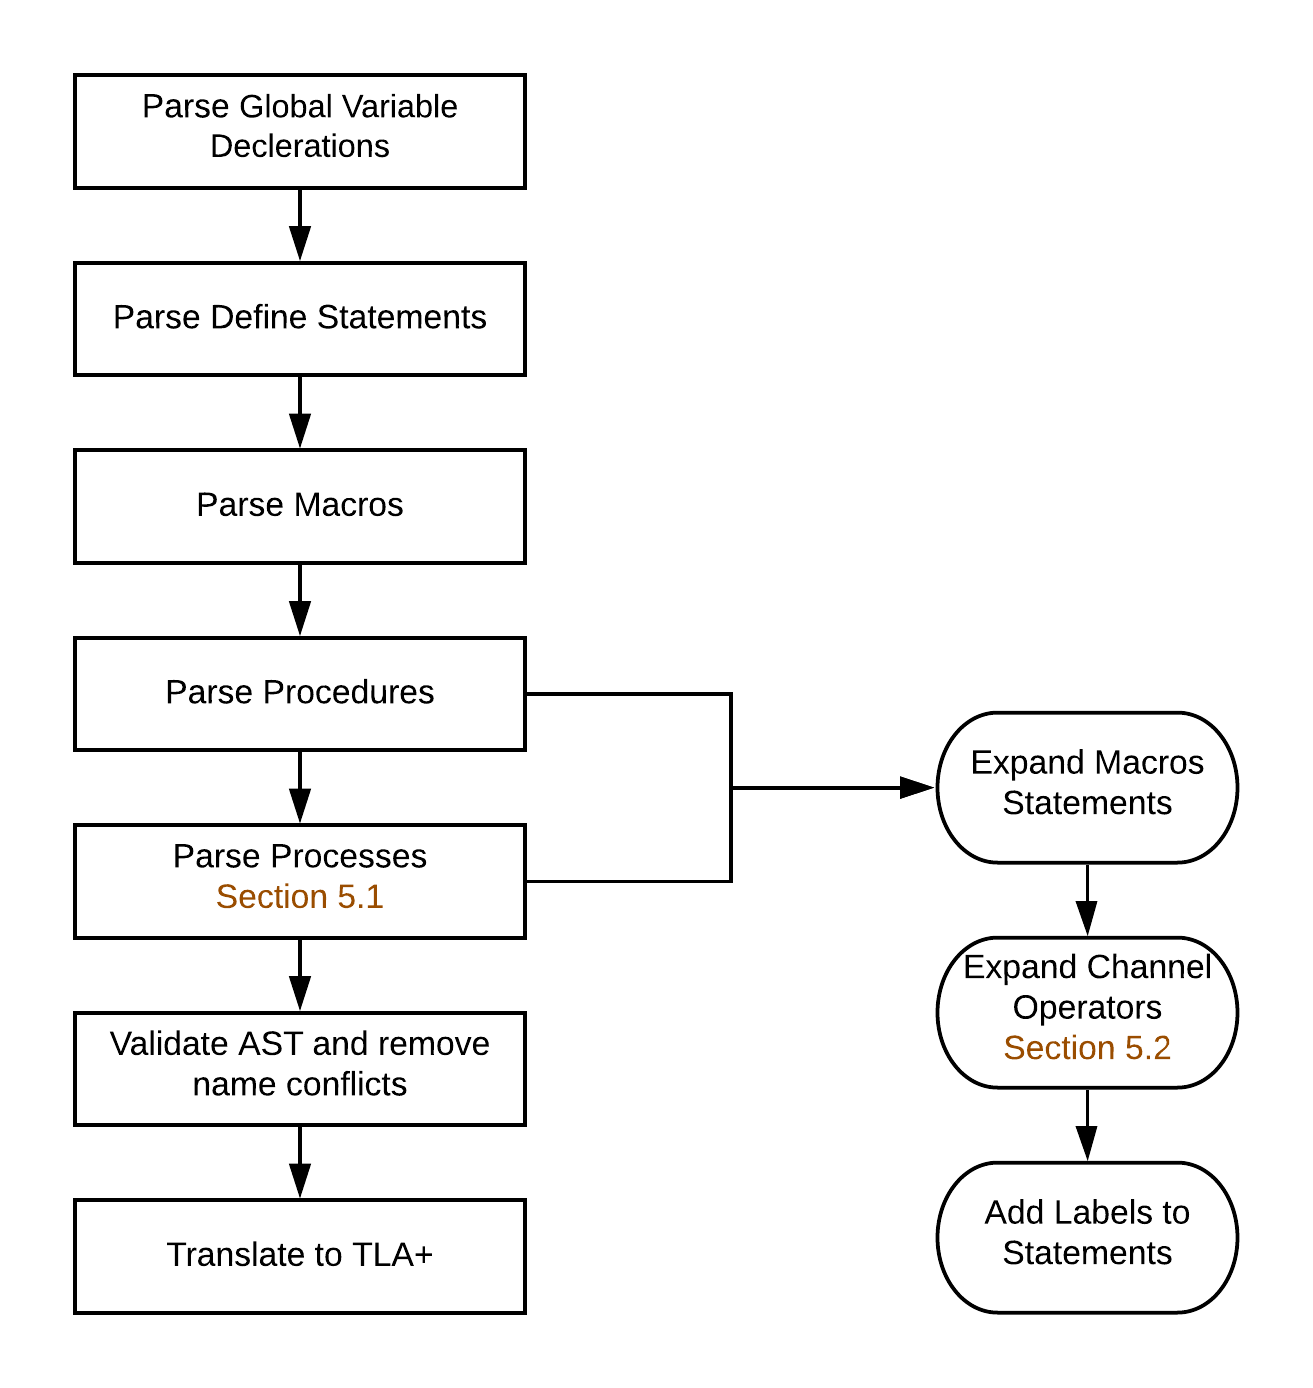
\includegraphics[width=0.7\textwidth]{chart}
\caption{Parsing tasks in Distributed PlusCal translator}
\end{figure}
\section{Parsing Processes}

When parsing a process, the translator distinguishes the sub-processes using sub-process separators. the separators differ based on the PlusCal syntax the programmer is using. In c-syntax PlusCal the sub-processes separators are curly brackets as explained in \ref{subProcess}.

Each block of statements read in a sub-process is placed in a vector of sub-processes. All of the statements are parsed and transformed into the appropriate structure with respect to the type of each statement, they are then placed in an AST(Abstract syntax tree) that represents the entire algorithm.

The AST includes statement types such as $if$ statements and $while$ statements. Our translator added more types to the AST to be able to hold sub-processes and channel operators.


Then the bodies of the sub-processes go through the expansion process described in \ref{translator} and \ref{chanexpand}.

\label{parsesub}
\section{Channel operator expansion}

The expansions refer to the process of structurally expanding code fragments during compilation. The PlusCal translator uses the expansion process to transform $Macro Calls$ that are within a statement to the body of the defined macro with the arguments the programmer has passed.

The expansion process deals with channel operators, so when a channel operator is found in a statement, the translator generates the appropriate template body corresponding to the channel operator used. when generating the expanded body of the operator the arguments used when calling the operator are substituted.

The expanded body is generated polymorphically based on the type of the channel, meaning the expanded body for a channel operator  depends on the type of channel that is passed as an argument with the operator.

For instance, consider the $receive$ operator in the two phase commit example
\[
receive(coord, msg)
\]

The listing below shows the statement before the expansion process as a part of the AST.

\begin{lstlisting}
[type |-> "ChannelReceiver",
channel |-> coord, targetVar |-> msg, callExp |-> <<  >>, targetExp |-> <<  >>]

\end{lstlisting}

The generated body template is based on the channel type and the operator, so the listing shown below is the template for a receive channel operator when receiving from an unordered channel.

\begin{lstlisting}
with(e \in chan){
	msg := e;
	chan := chan \ {e}
}
\end{lstlisting}

After applying the expansion process using this body template the AST is modified to hold the statements corresponding to the channel receive operator as shows below.

\begin{lstlisting}
[type   |-> "with", 
 var    |-> "c",
 eqOrIn |-> "\\in",
 exp    |-> << "coord" >>,
 do     |-> <<[type |-> "assignment",
               ass  |-> <<[lhs |-> [var |-> "msg", sub |-> <<  >>],
                           rhs |-> << "c" >>], 
                          [lhs |-> [var |-> "coord", sub |-> <<  >>],
                           rhs |-> << "coord", " \ ", "{", "c", "}" >>]>>]>>]

\end{lstlisting}

\label{chanexpand}
\chapter{Conclusion and future work}

This thesis presents Distributed PlusCal, an language extending PlusCal, with the goal of providing the user with constructs that support the modeling of distributed algorithms. We also provide a compiler from Distributed PlusCal to \tlaplus.

In the future we aim to introduce more types of communication channels, and we're working on supporting PlusCals p-syntax as well.

\begin{appendices}
\chapter{Distributed PlusCal to TLA+ Examples}
\label{appendix:examples}
\section{Two Phase Commit}

\begin{lstlisting}[caption = TLA+ translation for Sub-Processes, frame = tlrb, firstnumber = 1]

----------------------------- MODULE 2pc -----------------------------
EXTENDS Sequences, Naturals

CONSTANTS Coord, Agent

State == {"unknown", "accept", "refuse", "commit", "abort"}

    
(* PlusCal options (-distpcal) *)

(***
--algorithm TPC {
 
  \* message channels
  channels coord, agt[Agent];
     
  fair process (a \in Agent)
  variable aState = "unknown"; {

a1: if (aState = "unknown") {
        with(st \in {"accept", "refuse"}) {
          aState := st;
          send(coord, [type |-> st, agent |-> self]);
        };
    };
    a2: await(aState \in {"commit", "abort"})
    
  } {
    
    a3:await (aState # "unknown");
       receive(agt[self], aState); 
       
    a4:clear(agt);
  }

  fair process (c = Coord) 
  variables cState = "unknown",
            commits = {}, msg = {};
             \* agents that agree to commit
  {
    c1: await(cState \in {"commit", "abort"});    
        broadcast(agt, [ag \in Agent|-> cState]);
  } {
        
     c2:while (cState \notin {"abort", "commit"}) {
        receive(coord, msg);
            if (msg.type = "refuse") {
                cState := "abort";
            }
            else if (msg.type = "accept") {
                commits := commits \cup {msg.agent};
                 if (commits = Agent) {
                    cState := "commit";
                 }
              }
        }
  }
 }
***)
\* BEGIN TRANSLATION
VARIABLES coord, agt, pc, aState, cState, commits, msg

vars == << coord, agt, pc, aState, cState, commits, msg >>

ProcSet == (Agent) \cup {Coord}

SubProcSet == [n \in ProcSet |-> IF n \in Agent THEN 1..2
                             ELSE (**Coord**) 1..2]

Init == (* Global variables *)
        /\ coord = {}
        /\ agt = [a0 \in Agent |-> {}]
        (* Node a *)
        /\ aState = [self \in Agent |-> "unknown"]
        (* Node c *)
        /\ cState = "unknown"
        /\ commits = {}
        /\ msg = {}
        /\ pc = [self \in ProcSet |-> CASE self \in Agent -> <<"a1","a3">>
                                        [] self = Coord -> <<"c1","c2">>]

a1(self) == /\ pc[self] [1] = "a1"
            /\ IF aState[self] = "unknown"
                  THEN /\ \E st \in {"accept", "refuse"}:
                            /\ aState' = [aState EXCEPT ![self] = st]
                            /\ coord' = (coord \cup {[type |-> st, agent |-> self]})
                  ELSE /\ TRUE
                       /\ UNCHANGED << coord, aState >>
            /\ pc' = [pc EXCEPT ![self] = [@  EXCEPT ![1] = "a2"]]
            /\ UNCHANGED << agt, cState, commits, msg >>

a2(self) == /\ pc[self] [1] = "a2"
            /\ (aState[self] \in {"commit", "abort"})
            /\ pc' = [pc EXCEPT ![self] = [@  EXCEPT ![1] = "Done"]]
            /\ UNCHANGED << coord, agt, aState, cState, commits, msg >>

a3(self) == /\ pc[self] [2] = "a3"
            /\ (aState[self] # "unknown")
            /\ \E a1519 \in agt[self]:
                 /\ aState' = [aState EXCEPT ![self] = a1519]
                 /\ agt' = [agt EXCEPT ![self] = agt[self] \ {a1519}]
            /\ pc' = [pc EXCEPT ![self] = [@  EXCEPT ![2] = "a4"]]
            /\ UNCHANGED << coord, cState, commits, msg >>

a4(self) == /\ pc[self] [2] = "a4"
            /\ agt' = [a0 \in Agent |-> {}]
            /\ pc' = [pc EXCEPT ![self] = [@  EXCEPT ![2] = "Done"]]
            /\ UNCHANGED << coord, aState, cState, commits, msg >>

a(self) == a1(self) \/ a2(self) \/ a3(self) \/ a4(self)

c1 == /\ pc[Coord] [1] = "c1"
      /\ (cState \in {"commit", "abort"})
      /\ agt' = [ag \in Agent |-> agt[ag] \cup  {cState} ]
      /\ pc' = [pc EXCEPT ![Coord] = [@  EXCEPT ![1] = "Done"]]
      /\ UNCHANGED << coord, aState, cState, commits, msg >>

c2 == /\ pc[Coord] [2] = "c2"
      /\ IF cState \notin {"abort", "commit"}
            THEN /\ \E c1512 \in coord:
                      /\ coord' = coord \ {c1512}
                      /\ msg' = c1512
                 /\ IF msg'.type = "refuse"
                       THEN /\ cState' = "abort"
                            /\ UNCHANGED commits
                       ELSE /\ IF msg'.type = "accept"
                                  THEN /\ commits' = (commits \cup {msg'.agent})
                                       /\ IF commits' = Agent
                                             THEN /\ cState' = "commit"
                                             ELSE /\ TRUE
                                                  /\ UNCHANGED cState
                                  ELSE /\ TRUE
                                       /\ UNCHANGED << cState, commits >>
                 /\ pc' = [pc EXCEPT ![Coord] = [@  EXCEPT ![2] = "c2"]]
            ELSE /\ pc' = [pc EXCEPT ![Coord] = [@  EXCEPT ![2] = "Done"]]
                 /\ UNCHANGED << coord, cState, commits, msg >>
      /\ UNCHANGED << agt, aState >>

c == c1 \/ c2

(* Allow infinite stuttering to prevent deadlock on termination. *)
Terminating == /\ \A self \in ProcSet : \A sub \in SubProcSet[self]: pc[self][sub] = "Done"
               /\ UNCHANGED vars

Next == c
           \/ (\E self \in Agent: a(self))
           \/ Terminating

Spec == /\ Init /\ [][Next]_vars
        /\ \A self \in Agent : WF_vars(a(self))
        /\ WF_vars(c)

Termination == <>(\A self \in ProcSet: \A sub \in SubProcSet[self] : pc[self][sub] = "Done")

\* END TRANSLATION
=============================================================================

\end{lstlisting}

\section{Lamport Mutex}
\begin{lstlisting}[caption = TLA+ translation for Sub-Processes, frame = tlrb, firstnumber = 1]

---------------------------- MODULE lm ----------------------------

EXTENDS Naturals, Sequences, TLC

CONSTANT N

ASSUME N \in Nat 

Nodes == 1 .. N

(* PlusCal options (-distpcal) *)

(**
--algorithm LamportMutex {

   fifo network[Nodes, Nodes];
       
   define {
     Max(c,d) == IF c > d THEN c ELSE d
     \* messages used in the algorithm
     Request(c) == [type |-> "request", clock |-> c]
     Release(c) == [type |-> "release", clock |-> c]
     Acknowledge(c) == [type |-> "ack", clock |-> c]
   }
     
   process(n \in Nodes)
     variables clock = 0,
               req = [n \in Nodes |-> 0],
               ack = {},
               sndr, msg;
   {
      
     p0: while (TRUE) {
         p1:   skip;  \* non-critical section
         p2:   clock := clock + 1;

               \*sender is the specific node, receivers are all other nodes
               multicast(network, [self, nd \in Nodes |-> Request(clock)]);
               req[self] := clock;
               ack := {self};
               
         p3:   await (/\ ack = Nodes
                      /\ \A n \in Nodes \ {self} : \/ req[n] = 0
                                                   \/ req[self] < req[n]
                                                   \/ (self < n /\ req[self] = req[n]));

         cs:   skip;
         p4:   clock := clock + 1;
               multicast(network, [self, n \in Nodes \ {self} |-> Release(clock)]);
               
               \*to be used on the entire channel not sub-parts
               \* clear(network); \* if we want to add this add -label to the options
       } \* end while
   }{

rcv:
     while (TRUE) {
        with (n \in Nodes) {
           sndr := n;
           receive(network[n,self], msg);
           clock := Max(clock, msg.clock) + 1
        };
handle:
        if (msg.type = "request") {
           req[sndr] := msg.clock;
           
           send(network[self, sndr], Acknowledge(clock))
        }
        else if (msg.type = "ack") {
           ack := ack \cup {sndr};
        }
        else if (msg.type = "release") {
           req[sndr] := 0;
        }
     }  \* end while
   } 
}
**)
\* BEGIN TRANSLATION 

CONSTANT defaultInitValue
VARIABLES network, pc

(* define statement *)
Max(c,d) == IF c > d THEN c ELSE d

Request(c) == [type |-> "request", clock |-> c]
Release(c) == [type |-> "release", clock |-> c]
Acknowledge(c) == [type |-> "ack", clock |-> c]

VARIABLES clock, req, ack, sndr, msg

vars == << network, pc, clock, req, ack, sndr, msg >>

ProcSet == (Nodes)

SubProcSet == [n \in ProcSet |-> 1..2]

Init == (* Global variables *)
        /\ network = [n0 \in Nodes, n1 \in Nodes |-> <<>>]
        (* Node n *)
        /\ clock = [self \in Nodes |-> 0]
        /\ req = [self \in Nodes |-> [n \in Nodes |-> 0]]
        /\ ack = [self \in Nodes |-> {}]
        /\ sndr = [self \in Nodes |-> defaultInitValue]
        /\ msg = [self \in Nodes |-> defaultInitValue]
        /\ pc = [self \in ProcSet |-> <<"p0","rcv">>]

p0(self) == /\ pc[self] [1] = "p0"
            /\ pc' = [pc EXCEPT ![self] = [@  EXCEPT ![1] = "p1"]]
            /\ UNCHANGED << network, clock, req, ack, sndr, msg >>

p1(self) == /\ pc[self] [1] = "p1"
            /\ TRUE
            /\ pc' = [pc EXCEPT ![self] = [@  EXCEPT ![1] = "p2"]]
            /\ UNCHANGED << network, clock, req, ack, sndr, msg >>

p2(self) == /\ pc[self] [1] = "p2"
            /\ clock' = [clock EXCEPT ![self] = clock[self] + 1]
            /\ network' = [<<slf, nd>> \in DOMAIN network |->  IF slf = self 
                           /\ nd \in Nodes THEN 
                           Append(network[slf, nd], Request(clock'[self])) ELSE network[slf, nd]]
            /\ req' = [req EXCEPT ![self][self] = clock'[self]]
            /\ ack' = [ack EXCEPT ![self] = {self}]
            /\ pc' = [pc EXCEPT ![self] = [@  EXCEPT ![1] = "p3"]]
            /\ UNCHANGED << sndr, msg >>

p3(self) == /\ pc[self] [1] = "p3"
            /\ (/\ ack[self] = Nodes
                /\ \A n \in Nodes \ {self} : \/ req[self][n] = 0
                                             \/ req[self][self] < req[self][n]
                                             \/ (self < n /\ req[self][self] = req[self][n]))
            /\ pc' = [pc EXCEPT ![self] = [@  EXCEPT ![1] = "cs"]]
            /\ UNCHANGED << network, clock, req, ack, sndr, msg >>

cs(self) == /\ pc[self] [1] = "cs"
            /\ TRUE
            /\ pc' = [pc EXCEPT ![self] = [@  EXCEPT ![1] = "p4"]]
            /\ UNCHANGED << network, clock, req, ack, sndr, msg >>

p4(self) == /\ pc[self] [1] = "p4"
            /\ clock' = [clock EXCEPT ![self] = clock[self] + 1]
            /\ network' = [<<slf, n>> \in DOMAIN network |->  IF slf = self 
                           /\ n \in Nodes \ { self } THEN 
                           Append(network[slf, n], Release(clock'[self])) ELSE network[slf, n]]
            /\ pc' = [pc EXCEPT ![self] = [@  EXCEPT ![1] = "p0"]]
            /\ UNCHANGED << req, ack, sndr, msg >>

rcv(self) == /\ pc[self] [2] = "rcv"
             /\ \E n \in Nodes:
                  /\ sndr' = [sndr EXCEPT ![self] = n]
                  /\ Len(network[n,self]) > 0 
                  /\ msg' = [msg EXCEPT ![self] = Head(network[n,self])]
                  /\ network' = [network EXCEPT ![n,self] =  Tail(@) ]
                  /\ clock' = [clock EXCEPT ![self] = Max(clock[self], msg'[self].clock) + 1]
             /\ pc' = [pc EXCEPT ![self] = [@  EXCEPT ![2] = "handle"]]
             /\ UNCHANGED << req, ack >>

handle(self) == /\ pc[self] [2] = "handle"
                /\ IF msg[self].type = "request"
                      THEN /\ req' = [req EXCEPT ![self][sndr[self]] = msg[self].clock]
                           /\ network' = [network EXCEPT ![self, sndr[self]] =  Append(@, Acknowledge(clock[self]))]
                           /\ ack' = ack
                      ELSE /\ IF msg[self].type = "ack"
                                 THEN /\ ack' = [ack EXCEPT ![self] = ack[self] \cup {sndr[self]}]
                                      /\ req' = req
                                 ELSE /\ IF msg[self].type = "release"
                                            THEN /\ req' = [req EXCEPT ![self][sndr[self]] = 0]
                                            ELSE /\ TRUE
                                                 /\ req' = req
                                      /\ ack' = ack
                           /\ UNCHANGED network
                /\ pc' = [pc EXCEPT ![self] = [@  EXCEPT ![2] = "rcv"]]
                /\ UNCHANGED << clock, sndr, msg >>

n(self) == p0(self) \/ p1(self) \/ p2(self) \/ p3(self) \/ cs(self)
              \/ p4(self) \/ rcv(self) \/ handle(self)

Next == (\E self \in Nodes: n(self))

Spec == Init /\ [][Next]_vars

\* END TRANSLATION

=============================================================================

\end{lstlisting}

\end{appendices}

\bibliographystyle{alpha}
\bibliography{report}

\end{document}
